\documentclass[12pt,aspectratio=169]{beamer}
\usetheme{metropolis}
\setbeamersize{text margin left=.5cm,text margin right=.5cm}
\usepackage[lf]{carlito}
\usepackage{siunitx}
\usepackage{tikz}
\usepackage{mathpazo}
\usepackage{bm}
\usepackage{mathtools}
\usepackage[ISO]{diffcoeff}
\diffdef{}{ op-symbol=\mathsf{d} }
\usepackage{xcolor,colortbl}

%\usepackage[siunitx]{circuitikz} % to draw circuits!

\title{Class 19: Assymmetry in Faraday's Law}
\subtitle{Advanced Placement Physics C}
\author[TML]{Dr.\ Timothy Leung}
\institute{Olympiads School}
\date{Updated: Summer 2022}

\newcommand{\pic}[2]{
  \includegraphics[width=#1\textwidth]{#2}
}
\newcommand{\eq}[2]{
  \vspace{#1}{\Large
    \begin{displaymath}
      #2
    \end{displaymath}
  }
}
%\newcommand{\iii}{\ensuremath\hat{\bm{\imath}}}
%\newcommand{\jjj}{\ensuremath\hat{\bm{\jmath}}}
%\newcommand{\kkk}{\ensuremath\hat{\bm{k}}}
%\newcommand{\iii}{\ensuremath\hat x}
%\newcommand{\jjj}{\ensuremath\hat y}
%\newcommand{\kkk}{\ensuremath\hat z}



\begin{document}

\begin{frame}
  \maketitle
\end{frame}


\begin{frame}{A Coil Moving Through a Magnetic Field}
  A loop of wire moves through a magnetic field $\vec B$ into the page with
  velocity $\vec v$. From Faraday's law, when the wire moves \emph{into} the
  magnetic field, and when it moves \emph{out} of the field, magnetic flux
  $\Phi_m$ changes, creating an electromotive force $\mathcal E$:

  \eq{-.2in}{
    \boxed{ \mathcal E=-\diff{\Phi_m}t }
  }
  \begin{center}
    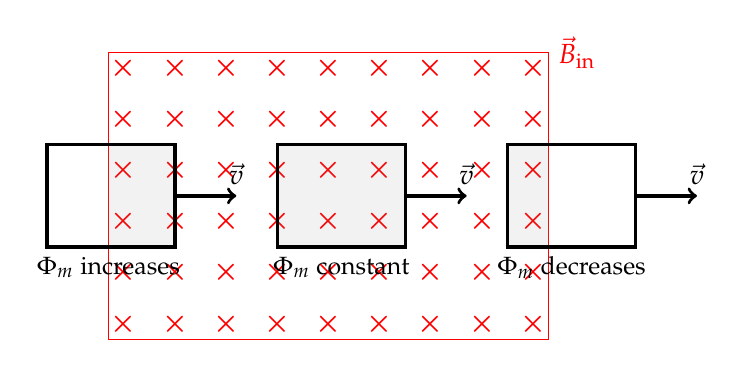
\begin{tikzpicture}[scale=.65]
      \draw[red](-.3,-.3) rectangle(8.3,5.3) node[right]{$\vec B_\text{in}$};
      \foreach\x in {0,1,...,8}{
        \foreach\y in {0,1,...,5}
        \node at (\x,\y) {\textcolor{red}{$\bm\times$}};
      }
      
      \fill[gray,opacity=.1](-.3,1.5) rectangle(1,3.5);
      \draw[very thick](-1.5,1.5) rectangle(1,3.5);
      \draw[very thick,->](1,2.5)--(2.2,2.5) node[above]{$\vec v$};
      \node[below] at (-.3,1.5) {\small $\Phi_m$ increases};

      \uncover<2->{
        \fill[gray,opacity=.1](3,1.5) rectangle(5.5,3.5);
        \draw[very thick](3,1.5) rectangle(5.5,3.5);
        \draw[very thick,->](5.5,2.5)--(6.7,2.5) node[above]{$\vec v$};
        \node[below] at (4.25,1.5) {\small $\Phi_m$ constant};
      }
      \uncover<3->{
        \fill[gray,opacity=.1](7.5,1.5) rectangle(8.3,3.5);
        \draw[very thick](7.5,1.5) rectangle(10,3.5);
        \draw[very thick,->](10,2.5)--(11.2,2.5) node[above]{$\vec v$};
        \node[below] at (8.75,1.5) {\small $\Phi_m$ decreases};
      }
    \end{tikzpicture}
  \end{center}

  \vspace{-.1in}

\end{frame}



\begin{frame}{Coil Moving Through a Magnetic Field}
  For an observer in the same frame of reference as the magnetic field, the
  reason is obvious. The charges\footnote{presumably positive, but it doesn't
    really matter} inside the wire experience a \emph{magnetic force} as they
  move through the magnetic field, creating an \emph{emf}, and an electric
  current. This is called \textbf{motional EMF}.
  \begin{center}
    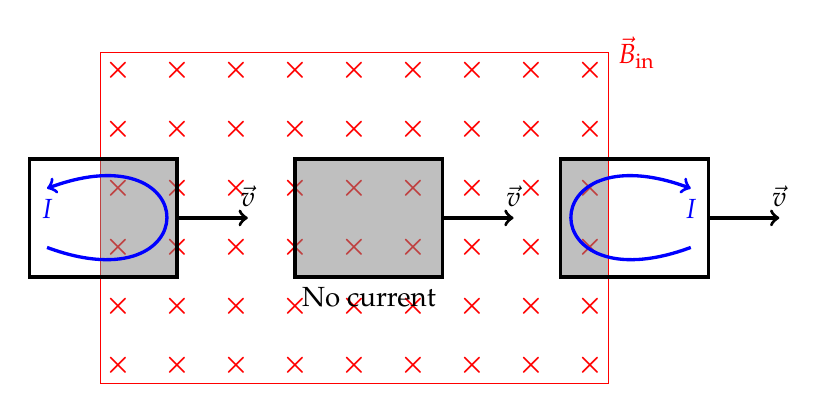
\begin{tikzpicture}[scale=.75]
      \draw[red](-.3,-.3) rectangle(8.3,5.3) node[right]{$\vec B_\text{in}$};
      \foreach\x in {0,1,...,8}{
        \foreach\y in {0,1,...,5}
        \node at (\x,\y) {\textcolor{red}{$\bm\times$}};
      }
      
      \fill[gray,opacity=.5](-.3,1.5) rectangle(1,3.5);
      \draw[very thick](-1.5,1.5) rectangle(1,3.5);
      \draw[very thick,->](1,2.5)--(2.2,2.5) node[above]{$\vec v$};
      \draw[very thick,->,blue](-1.2,2)..controls(1.5,1) and (1.5,4)..(-1.2,3)
      node[below]{$I$};

      \uncover<2->{
        \fill[gray,opacity=.5](3,1.5) rectangle(5.5,3.5);
        \draw[very thick](3,1.5) rectangle(5.5,3.5);
        \draw[very thick,->](5.5,2.5)--(6.7,2.5) node[above]{$\vec v$};
        \node[below] at (4.25,1.5) {No current};
      }
      \uncover<3->{
        \fill[gray,opacity=.5](7.5,1.5) rectangle(8.3,3.5);
        \draw[very thick](7.5,1.5) rectangle(10,3.5);
        \draw[very thick,->](10,2.5)--(11.2,2.5) node[above]{$\vec v$};
        \draw[very thick,->,blue](9.7,2)..controls(7,1) and (7,4)..(9.7,3)
        node[below]{$I$};
      }
    \end{tikzpicture}
  \end{center}
  \vspace{.2in}
\end{frame}




\begin{frame}{Magnetic Field Moving Past a Coil of Wire}
  For an observer in the same frame of reference as the wire, the reason is
  also obvious. As the magnetic field moves, the magnetic flux changes, and an
  \emph{electric field} is created in the wire. A current is created because
  the charges inside the wire experience an \emph{electric force}.
  \begin{center}
    \vspace{-.15in}
    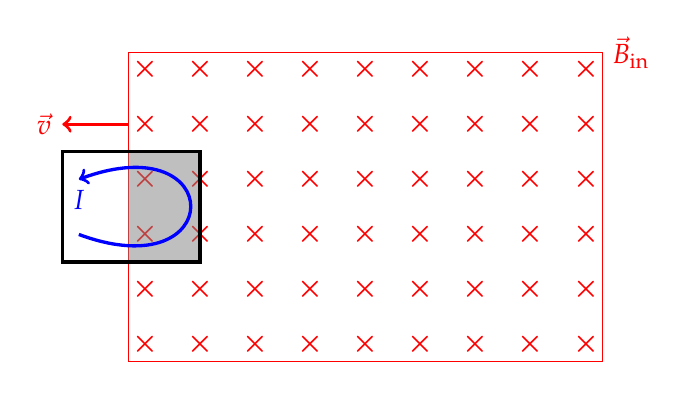
\begin{tikzpicture}[scale=.7]
      \draw[red](-.3,-.3) rectangle(8.3,5.3) node[right]{$\vec B_\text{in}$};
      \draw[red,very thick,->](-.3,4)--(-1.5,4) node[left]{$\vec v$};
      \foreach\x in {0,1,...,8}{
        \foreach\y in {0,1,...,5}
        \node at (\x,\y) {\textcolor{red}{$\bm\times$}};
      }
      
      \fill[gray,opacity=.5](-.3,1.5) rectangle(1,3.5);
      \draw[very thick](-1.5,1.5) rectangle(1,3.5);
      \draw[very thick,->,blue](-1.2,2)..controls(1.5,1) and (1.5,4)..(-1.2,3)
      node[below]{$I$};
    \end{tikzpicture}
  \end{center}
\end{frame}


\begin{frame}{Assymmetry in Faraday's Law}
  Both observers obtain the same result (same $\mathcal E$ and same current $I$
  in the wire), however they cannot agree on the \emph{reason}
\end{frame}
\end{document}
